\documentclass{book}
\usepackage[a4paper,top=2.5cm,bottom=2.5cm,left=2.5cm,right=2.5cm]{geometry}
\usepackage{makeidx}
\usepackage{natbib}
\usepackage{graphicx}
\usepackage{multicol}
\usepackage{float}
\usepackage{listings}
\usepackage{color}
\usepackage{ifthen}
\usepackage[table]{xcolor}
\usepackage{textcomp}
\usepackage{alltt}
\usepackage{ifpdf}
\ifpdf
\usepackage[pdftex,
            pagebackref=true,
            colorlinks=true,
            linkcolor=blue,
            unicode
           ]{hyperref}
\else
\usepackage[ps2pdf,
            pagebackref=true,
            colorlinks=true,
            linkcolor=blue,
            unicode
           ]{hyperref}
\usepackage{pspicture}
\fi
\usepackage[utf8]{inputenc}
\usepackage{mathptmx}
\usepackage[scaled=.90]{helvet}
\usepackage{courier}
\usepackage{sectsty}
\usepackage{amssymb}
\usepackage[titles]{tocloft}
\usepackage{doxygen}
\lstset{language=C++,inputencoding=utf8,basicstyle=\footnotesize,breaklines=true,breakatwhitespace=true,tabsize=4,numbers=left }
\makeindex
\setcounter{tocdepth}{3}
\renewcommand{\footrulewidth}{0.4pt}
\renewcommand{\familydefault}{\sfdefault}
\hfuzz=15pt
\setlength{\emergencystretch}{15pt}
\hbadness=750
\tolerance=750
\begin{document}
\hypersetup{pageanchor=false,citecolor=blue}
\begin{titlepage}
\vspace*{7cm}
\begin{center}
{\Large class\-\_\-image \\[1ex]\large version 1 }\\
\vspace*{1cm}
{\large Generated by Doxygen 1.8.3.1}\\
\vspace*{0.5cm}
{\small Thu Feb 28 2013 11:09:58}\\
\end{center}
\end{titlepage}
\clearemptydoublepage
\pagenumbering{roman}
\tableofcontents
\clearemptydoublepage
\pagenumbering{arabic}
\hypersetup{pageanchor=true,citecolor=blue}
\chapter{Hierarchical Index}
\section{Class Hierarchy}
This inheritance list is sorted roughly, but not completely, alphabetically\-:\begin{DoxyCompactList}
\item \contentsline{section}{Generic\-Images\-Downloader}{\pageref{class_generic_images_downloader}}{}
\begin{DoxyCompactList}
\item \contentsline{section}{Google\-Image\-Downloader}{\pageref{class_google_image_downloader}}{}
\item \contentsline{section}{Imagebase\-Downloader}{\pageref{class_imagebase_downloader}}{}
\item \contentsline{section}{Office\-Image\-Downloader}{\pageref{class_office_image_downloader}}{}
\item \contentsline{section}{Photo\-Bucket\-Downloader}{\pageref{class_photo_bucket_downloader}}{}
\item \contentsline{section}{Rgb\-Stock\-Image\-Downloader}{\pageref{class_rgb_stock_image_downloader}}{}
\end{DoxyCompactList}
\item \contentsline{section}{Google\-Image}{\pageref{class_google_image}}{}
\end{DoxyCompactList}

\chapter{Data Structure Index}
\section{Data Structures}
Here are the data structures with brief descriptions\-:\begin{DoxyCompactList}
\item\contentsline{section}{\hyperlink{class_generic_images_downloader}{Generic\-Images\-Downloader} \\*Cette classe est la classe générique à toutes les auutres }{\pageref{class_generic_images_downloader}}{}
\item\contentsline{section}{\hyperlink{class_google_image}{Google\-Image} \\*Cette classe permet de télécharger les images des résultats de \char`\"{}\-Google Image\char`\"{} }{\pageref{class_google_image}}{}
\item\contentsline{section}{\hyperlink{class_google_image_downloader}{Google\-Image\-Downloader} \\*Cette classe permet de télécharger les images des résultats de \char`\"{}\-Google Image\char`\"{} }{\pageref{class_google_image_downloader}}{}
\item\contentsline{section}{\hyperlink{class_imagebase_downloader}{Imagebase\-Downloader} \\*Cette classe permet de télécharger les images des résultats de \char`\"{}imagebase.\-net\char`\"{} }{\pageref{class_imagebase_downloader}}{}
\item\contentsline{section}{\hyperlink{class_office_image_downloader}{Office\-Image\-Downloader} \\*Cette classe permet de télécharger les images des résultats de \char`\"{}\-Office.\-microsoft.\-com\char`\"{} }{\pageref{class_office_image_downloader}}{}
\item\contentsline{section}{\hyperlink{class_photo_bucket_downloader}{Photo\-Bucket\-Downloader} \\*Cette classe permet de télécharger les images des résultats de \char`\"{}photobucket.\-com\char`\"{} }{\pageref{class_photo_bucket_downloader}}{}
\item\contentsline{section}{\hyperlink{class_rgb_stock_image_downloader}{Rgb\-Stock\-Image\-Downloader} \\*Cette classe permet de télécharger les images des résultats de \char`\"{}rgbstock.\-com\char`\"{} }{\pageref{class_rgb_stock_image_downloader}}{}
\end{DoxyCompactList}

\chapter{File Index}
\section{File List}
Here is a list of all documented files with brief descriptions\-:\begin{DoxyCompactList}
\item\contentsline{section}{\hyperlink{_generic_images_downloader_8class_8php}{Generic\-Images\-Downloader.\-class.\-php} \\*\hyperlink{class_generic_images_downloader}{Generic\-Images\-Downloader} class file }{\pageref{_generic_images_downloader_8class_8php}}{}
\item\contentsline{section}{\hyperlink{googleimage_8class_8php}{googleimage.\-class.\-php} \\*\hyperlink{class_google_image}{Google\-Image} class file }{\pageref{googleimage_8class_8php}}{}
\item\contentsline{section}{\hyperlink{_google_image_downloader_8class_8php}{Google\-Image\-Downloader.\-class.\-php} \\*\hyperlink{class_google_image_downloader}{Google\-Image\-Downloader} class file }{\pageref{_google_image_downloader_8class_8php}}{}
\item\contentsline{section}{\hyperlink{_image_base_downloader_8class_8php}{Image\-Base\-Downloader.\-class.\-php} \\*\hyperlink{class_imagebase_downloader}{Imagebase\-Downloader} class file }{\pageref{_image_base_downloader_8class_8php}}{}
\item\contentsline{section}{\hyperlink{_office_image_downloader_8class_8php}{Office\-Image\-Downloader.\-class.\-php} \\*\hyperlink{class_office_image_downloader}{Office\-Image\-Downloader} class file }{\pageref{_office_image_downloader_8class_8php}}{}
\item\contentsline{section}{\hyperlink{_photo_bucket_downloader_8class_8php}{Photo\-Bucket\-Downloader.\-class.\-php} \\*\hyperlink{class_photo_bucket_downloader}{Photo\-Bucket\-Downloader} class file }{\pageref{_photo_bucket_downloader_8class_8php}}{}
\item\contentsline{section}{\hyperlink{_rgb_stock_image_downloader_8class_8php}{Rgb\-Stock\-Image\-Downloader.\-class.\-php} \\*\hyperlink{class_rgb_stock_image_downloader}{Rgb\-Stock\-Image\-Downloader} class file }{\pageref{_rgb_stock_image_downloader_8class_8php}}{}
\end{DoxyCompactList}

\chapter{Data Structure Documentation}
\hypertarget{class_generic_images_downloader}{\section{Generic\-Images\-Downloader Class Reference}
\label{class_generic_images_downloader}\index{Generic\-Images\-Downloader@{Generic\-Images\-Downloader}}
}


Cette classe est la classe générique à toutes les auutres.  


Inheritance diagram for Generic\-Images\-Downloader\-:\begin{figure}[H]
\begin{center}
\leavevmode
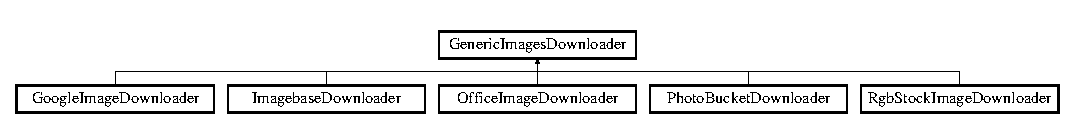
\includegraphics[height=1.287356cm]{class_generic_images_downloader}
\end{center}
\end{figure}
\subsection*{Public Member Functions}
\begin{DoxyCompactItemize}
\item 
\hyperlink{class_generic_images_downloader_a1df9ccba19fdd7050e21d302c7f58d35}{\-\_\-\-\_\-construct} (\$domain, \$path)
\begin{DoxyCompactList}\small\item\em Le constructeur. \end{DoxyCompactList}\item 
\hyperlink{class_generic_images_downloader_aeaf78020730e78dd35d16d14b527b44c}{search} (array \&\$errors=array())
\begin{DoxyCompactList}\small\item\em Déclaration de la fonction recherche. \end{DoxyCompactList}\item 
\hyperlink{class_generic_images_downloader_a3813247f2eae6ac65a8a021daf05bae4}{get\-Results} ()
\begin{DoxyCompactList}\small\item\em Retourne le tableau d'images. \end{DoxyCompactList}\item 
\hyperlink{class_generic_images_downloader_ae56b5f60923f542064ba1aae8b2af268}{set\-Pagination} (\$nb\-Result)
\begin{DoxyCompactList}\small\item\em Prépare la pagination. \end{DoxyCompactList}\item 
\hypertarget{class_generic_images_downloader_a421831a265621325e1fdd19aace0c758}{\hyperlink{class_generic_images_downloader_a421831a265621325e1fdd19aace0c758}{\-\_\-\-\_\-destruct} ()}\label{class_generic_images_downloader_a421831a265621325e1fdd19aace0c758}

\begin{DoxyCompactList}\small\item\em Détruit la classe. \end{DoxyCompactList}\end{DoxyCompactItemize}
\subsection*{Data Fields}
\begin{DoxyCompactItemize}
\item 
\hypertarget{class_generic_images_downloader_a3982e7af9d3327658dc69aec5fbee4d4}{const \hyperlink{class_generic_images_downloader_a3982e7af9d3327658dc69aec5fbee4d4}{N\-O\-\_\-\-K\-E\-Y\-W\-O\-R\-D\-S} = 1}\label{class_generic_images_downloader_a3982e7af9d3327658dc69aec5fbee4d4}

\begin{DoxyCompactList}\small\item\em Erreur aucun mot clé. \end{DoxyCompactList}\item 
\hypertarget{class_generic_images_downloader_a2ab25e02418e0ec9055aa6d8cfe25383}{const \hyperlink{class_generic_images_downloader_a2ab25e02418e0ec9055aa6d8cfe25383}{N\-O\-\_\-\-R\-E\-S\-U\-L\-T\-A\-T\-\_\-\-N\-U\-M\-B\-E\-R} = 2}\label{class_generic_images_downloader_a2ab25e02418e0ec9055aa6d8cfe25383}

\begin{DoxyCompactList}\small\item\em Erreur aucun nombre de résultat maximum introduit. \end{DoxyCompactList}\item 
\hypertarget{class_generic_images_downloader_a402bb789cf5cda26705e575ff3f84072}{const \hyperlink{class_generic_images_downloader_a402bb789cf5cda26705e575ff3f84072}{N\-O\-\_\-\-C\-O\-N\-T\-E\-N\-T} = 3}\label{class_generic_images_downloader_a402bb789cf5cda26705e575ff3f84072}

\begin{DoxyCompactList}\small\item\em Erreur aucun contenu trouver. \end{DoxyCompactList}\item 
\hypertarget{class_generic_images_downloader_a5addbab3d5ba0a46bac11e752aff34f3}{const \hyperlink{class_generic_images_downloader_a5addbab3d5ba0a46bac11e752aff34f3}{S\-T\-A\-R\-T\-\_\-\-B\-L\-O\-C\-K\-\_\-\-N\-O\-T\-\_\-\-F\-O\-U\-N\-D} = 4}\label{class_generic_images_downloader_a5addbab3d5ba0a46bac11e752aff34f3}

\begin{DoxyCompactList}\small\item\em Erreur début du bloc non trouver. \end{DoxyCompactList}\item 
\hypertarget{class_generic_images_downloader_a72cb2b05f3c0320f799874ba521128b3}{const \hyperlink{class_generic_images_downloader_a72cb2b05f3c0320f799874ba521128b3}{E\-N\-D\-\_\-\-B\-L\-O\-C\-K\-\_\-\-N\-O\-T\-\_\-\-F\-O\-U\-N\-D} = 5}\label{class_generic_images_downloader_a72cb2b05f3c0320f799874ba521128b3}

\begin{DoxyCompactList}\small\item\em Erreur fin du bloc non trouver. \end{DoxyCompactList}\item 
\hypertarget{class_generic_images_downloader_aa6db587586065f8e2cc80947844b19bc}{const \hyperlink{class_generic_images_downloader_aa6db587586065f8e2cc80947844b19bc}{I\-N\-V\-A\-L\-I\-D\-\_\-\-R\-E\-G\-E\-X} = 6}\label{class_generic_images_downloader_aa6db587586065f8e2cc80947844b19bc}

\begin{DoxyCompactList}\small\item\em Erreur pas de donnée retournée par la regex. \end{DoxyCompactList}\end{DoxyCompactItemize}
\subsection*{Protected Member Functions}
\begin{DoxyCompactItemize}
\item 
\hyperlink{class_generic_images_downloader_a90110a2b38b48e2ffd2a907bb7e06e3c}{set\-Keywords} (\$keywords)
\begin{DoxyCompactList}\small\item\em Fonction traitant les mots cles afin de les prépare pour la recherche. \end{DoxyCompactList}\item 
\hypertarget{class_generic_images_downloader_a3a3e8ed69a7a72d69950426ec9424a64}{\hyperlink{class_generic_images_downloader_a3a3e8ed69a7a72d69950426ec9424a64}{build\-U\-R\-L} ()}\label{class_generic_images_downloader_a3a3e8ed69a7a72d69950426ec9424a64}

\begin{DoxyCompactList}\small\item\em Fonction permettant la création de l'U\-R\-L. \end{DoxyCompactList}\item 
\hyperlink{class_generic_images_downloader_a52c22363fbbda749c84c270a471f904e}{get\-Content} (\$url)
\begin{DoxyCompactList}\small\item\em Fonction exécutant la recherche du contenu depuis l'U\-R\-L donnée. \end{DoxyCompactList}\end{DoxyCompactItemize}
\subsection*{Protected Attributes}
\begin{DoxyCompactItemize}
\item 
\hypertarget{class_generic_images_downloader_a233d12bd8b6d3453e9a7a3f0b8c31db2}{\hyperlink{class_generic_images_downloader_a233d12bd8b6d3453e9a7a3f0b8c31db2}{\$results} = array()}\label{class_generic_images_downloader_a233d12bd8b6d3453e9a7a3f0b8c31db2}

\begin{DoxyCompactList}\small\item\em \$results Tableau contenant les résultats obtenus \end{DoxyCompactList}\item 
\hypertarget{class_generic_images_downloader_aef9cf198312d2f89238a8e8e2f0f67f3}{\hyperlink{class_generic_images_downloader_aef9cf198312d2f89238a8e8e2f0f67f3}{\$domain} = null}\label{class_generic_images_downloader_aef9cf198312d2f89238a8e8e2f0f67f3}

\begin{DoxyCompactList}\small\item\em \$domain Contient l'url du site \end{DoxyCompactList}\item 
\hypertarget{class_generic_images_downloader_a0a4baf0b22973c07685c3981f0d17fc4}{\hyperlink{class_generic_images_downloader_a0a4baf0b22973c07685c3981f0d17fc4}{\$path} = null}\label{class_generic_images_downloader_a0a4baf0b22973c07685c3981f0d17fc4}

\begin{DoxyCompactList}\small\item\em \$path Chemin relatif permettant la recherche \end{DoxyCompactList}\item 
\hypertarget{class_generic_images_downloader_a9fbd95bfcdf27d802a8c7938529a61ba}{\hyperlink{class_generic_images_downloader_a9fbd95bfcdf27d802a8c7938529a61ba}{\$keywords} = null}\label{class_generic_images_downloader_a9fbd95bfcdf27d802a8c7938529a61ba}

\begin{DoxyCompactList}\small\item\em \$keywords Chaine de caractères comportant les mots clés \end{DoxyCompactList}\item 
\hypertarget{class_generic_images_downloader_ad9721caaec06f589accb445e1679fb2b}{\hyperlink{class_generic_images_downloader_ad9721caaec06f589accb445e1679fb2b}{\$num\-Page} = 1}\label{class_generic_images_downloader_ad9721caaec06f589accb445e1679fb2b}

\begin{DoxyCompactList}\small\item\em \$numpage Contient le nombre de pages à parcourir \end{DoxyCompactList}\item 
\hypertarget{class_generic_images_downloader_a2e15ac624477c6e5fa77444ae4e269f8}{\hyperlink{class_generic_images_downloader_a2e15ac624477c6e5fa77444ae4e269f8}{\$curl} = null}\label{class_generic_images_downloader_a2e15ac624477c6e5fa77444ae4e269f8}

\begin{DoxyCompactList}\small\item\em \$curl Contiennent toutes les informations utiles à la fonction curl \end{DoxyCompactList}\item 
\hypertarget{class_generic_images_downloader_afe2428ced622c4fc3c144fab982de9d0}{\hyperlink{class_generic_images_downloader_afe2428ced622c4fc3c144fab982de9d0}{\$nb\-Result} = 20}\label{class_generic_images_downloader_afe2428ced622c4fc3c144fab982de9d0}

\begin{DoxyCompactList}\small\item\em \$nb\-Result Nombre de resultat demander \end{DoxyCompactList}\end{DoxyCompactItemize}


\subsection{Detailed Description}
Cette classe est la classe générique à toutes les auutres. 

\begin{DoxyAuthor}{Author}
M. D. (\href{mailto:mikanono01@hotmail.com}{\tt mikanono01@hotmail.\-com}) 
\end{DoxyAuthor}
\begin{DoxyVersion}{Version}
1 (27/02/2013) 
\end{DoxyVersion}


\subsection{Constructor \& Destructor Documentation}
\hypertarget{class_generic_images_downloader_a1df9ccba19fdd7050e21d302c7f58d35}{\index{Generic\-Images\-Downloader@{Generic\-Images\-Downloader}!\-\_\-\-\_\-construct@{\-\_\-\-\_\-construct}}
\index{\-\_\-\-\_\-construct@{\-\_\-\-\_\-construct}!GenericImagesDownloader@{Generic\-Images\-Downloader}}
\subsubsection[{\-\_\-\-\_\-construct}]{\setlength{\rightskip}{0pt plus 5cm}\-\_\-\-\_\-construct (
\begin{DoxyParamCaption}
\item[{}]{\$domain, }
\item[{}]{\$path}
\end{DoxyParamCaption}
)}}\label{class_generic_images_downloader_a1df9ccba19fdd7050e21d302c7f58d35}


Le constructeur. 


\begin{DoxyParams}{Parameters}
{\em \$domain} & U\-R\-L du site \\
\hline
{\em \$path} & Chemin relatif permettant la recherche\\
\hline
\end{DoxyParams}
Initialisation de curl 

\subsection{Member Function Documentation}
\hypertarget{class_generic_images_downloader_a52c22363fbbda749c84c270a471f904e}{\index{Generic\-Images\-Downloader@{Generic\-Images\-Downloader}!get\-Content@{get\-Content}}
\index{get\-Content@{get\-Content}!GenericImagesDownloader@{Generic\-Images\-Downloader}}
\subsubsection[{get\-Content}]{\setlength{\rightskip}{0pt plus 5cm}get\-Content (
\begin{DoxyParamCaption}
\item[{}]{\$url}
\end{DoxyParamCaption}
)\hspace{0.3cm}{\ttfamily [protected]}}}\label{class_generic_images_downloader_a52c22363fbbda749c84c270a471f904e}


Fonction exécutant la recherche du contenu depuis l'U\-R\-L donnée. 


\begin{DoxyParams}{Parameters}
{\em \$url} & U\-R\-L complète du site sur laquelle la recherche doit s'effectuer. \\
\hline
\end{DoxyParams}
\hypertarget{class_generic_images_downloader_a3813247f2eae6ac65a8a021daf05bae4}{\index{Generic\-Images\-Downloader@{Generic\-Images\-Downloader}!get\-Results@{get\-Results}}
\index{get\-Results@{get\-Results}!GenericImagesDownloader@{Generic\-Images\-Downloader}}
\subsubsection[{get\-Results}]{\setlength{\rightskip}{0pt plus 5cm}get\-Results (
\begin{DoxyParamCaption}
{}
\end{DoxyParamCaption}
)}}\label{class_generic_images_downloader_a3813247f2eae6ac65a8a021daf05bae4}


Retourne le tableau d'images. 

\begin{DoxyReturn}{Returns}
Un tableau associatif structuré de cette manière \-: array(\char`\"{}title\char`\"{}, \char`\"{}image\char`\"{} =$>$ array(\char`\"{}thumb\-\_\-url\char`\"{}, \char`\"{}url\char`\"{}, \char`\"{}alt\char`\"{}, \char`\"{}width\char`\"{}, \char`\"{}height\char`\"{})) 
\end{DoxyReturn}
\hypertarget{class_generic_images_downloader_aeaf78020730e78dd35d16d14b527b44c}{\index{Generic\-Images\-Downloader@{Generic\-Images\-Downloader}!search@{search}}
\index{search@{search}!GenericImagesDownloader@{Generic\-Images\-Downloader}}
\subsubsection[{search}]{\setlength{\rightskip}{0pt plus 5cm}search (
\begin{DoxyParamCaption}
\item[{array \&}]{\$errors = {\ttfamily array()}}
\end{DoxyParamCaption}
)\hspace{0.3cm}{\ttfamily [abstract]}}}\label{class_generic_images_downloader_aeaf78020730e78dd35d16d14b527b44c}


Déclaration de la fonction recherche. 


\begin{DoxyParams}{Parameters}
{\em \$errors} & Un tableau servant a affiché les possibles erreurs. \\
\hline
\end{DoxyParams}
\hypertarget{class_generic_images_downloader_a90110a2b38b48e2ffd2a907bb7e06e3c}{\index{Generic\-Images\-Downloader@{Generic\-Images\-Downloader}!set\-Keywords@{set\-Keywords}}
\index{set\-Keywords@{set\-Keywords}!GenericImagesDownloader@{Generic\-Images\-Downloader}}
\subsubsection[{set\-Keywords}]{\setlength{\rightskip}{0pt plus 5cm}set\-Keywords (
\begin{DoxyParamCaption}
\item[{}]{\$keywords}
\end{DoxyParamCaption}
)\hspace{0.3cm}{\ttfamily [protected]}}}\label{class_generic_images_downloader_a90110a2b38b48e2ffd2a907bb7e06e3c}


Fonction traitant les mots cles afin de les prépare pour la recherche. 


\begin{DoxyParams}{Parameters}
{\em \$keywords} & Chaine de caractères comportant les mots clés. \\
\hline
\end{DoxyParams}
\hypertarget{class_generic_images_downloader_ae56b5f60923f542064ba1aae8b2af268}{\index{Generic\-Images\-Downloader@{Generic\-Images\-Downloader}!set\-Pagination@{set\-Pagination}}
\index{set\-Pagination@{set\-Pagination}!GenericImagesDownloader@{Generic\-Images\-Downloader}}
\subsubsection[{set\-Pagination}]{\setlength{\rightskip}{0pt plus 5cm}set\-Pagination (
\begin{DoxyParamCaption}
\item[{}]{\$nb\-Result}
\end{DoxyParamCaption}
)}}\label{class_generic_images_downloader_ae56b5f60923f542064ba1aae8b2af268}


Prépare la pagination. 


\begin{DoxyParams}{Parameters}
{\em \$nb\-Result} & Nombre de résultat a afficher. \\
\hline
\end{DoxyParams}


The documentation for this class was generated from the following file\-:\begin{DoxyCompactItemize}
\item 
\hyperlink{_generic_images_downloader_8class_8php}{Generic\-Images\-Downloader.\-class.\-php}\end{DoxyCompactItemize}

\hypertarget{class_google_image}{\section{Google\-Image Class Reference}
\label{class_google_image}\index{Google\-Image@{Google\-Image}}
}


Cette classe permet de télécharger les images des résultats de \char`\"{}\-Google Image\char`\"{}.  


\subsection*{Public Member Functions}
\begin{DoxyCompactItemize}
\item 
\hyperlink{class_google_image_a5be5a913d3ed0858d381c321b468ed76}{\-\_\-\-\_\-construct} (\$size=self\-::\-S\-I\-Z\-E\-\_\-\-A\-L\-L, \$disable\-Safe\-Search=false, \$domain=null, \$lang=null, \$coding=null)
\begin{DoxyCompactList}\small\item\em Le constructeur. \end{DoxyCompactList}\item 
\hyperlink{class_google_image_a0d624b549023221829714196e71f38da}{search} (\$search)
\begin{DoxyCompactList}\small\item\em Débute une recherche sur google image. \end{DoxyCompactList}\item 
\hyperlink{class_google_image_a3813247f2eae6ac65a8a021daf05bae4}{get\-Results} ()
\begin{DoxyCompactList}\small\item\em Retourne le tableau d'images. \end{DoxyCompactList}\end{DoxyCompactItemize}
\subsection*{Data Fields}
\begin{DoxyCompactItemize}
\item 
\hypertarget{class_google_image_abafee20a240b78759837b9ecdc6a8ee1}{const \hyperlink{class_google_image_abafee20a240b78759837b9ecdc6a8ee1}{S\-I\-Z\-E\-\_\-\-A\-L\-L} = 0}\label{class_google_image_abafee20a240b78759837b9ecdc6a8ee1}

\begin{DoxyCompactList}\small\item\em Toutes les tailles. \end{DoxyCompactList}\item 
\hypertarget{class_google_image_a161af60b05bf26e7a5077178c3b4b5b6}{const \hyperlink{class_google_image_a161af60b05bf26e7a5077178c3b4b5b6}{S\-I\-Z\-E\-\_\-\-I\-C\-O\-N} = 1}\label{class_google_image_a161af60b05bf26e7a5077178c3b4b5b6}

\begin{DoxyCompactList}\small\item\em Tailles de type icône de bureau. \end{DoxyCompactList}\item 
\hypertarget{class_google_image_a0951e5a9a339649b79e8eeb68fbc21e8}{const \hyperlink{class_google_image_a0951e5a9a339649b79e8eeb68fbc21e8}{S\-I\-Z\-E\-\_\-\-M\-E\-D\-I\-U\-M} = 2}\label{class_google_image_a0951e5a9a339649b79e8eeb68fbc21e8}

\begin{DoxyCompactList}\small\item\em Tailles moyennes. \end{DoxyCompactList}\item 
\hypertarget{class_google_image_a16c410ead77a2d9ffe8e57980323543e}{const \hyperlink{class_google_image_a16c410ead77a2d9ffe8e57980323543e}{S\-I\-Z\-E\-\_\-\-L\-A\-R\-G\-E} = 3}\label{class_google_image_a16c410ead77a2d9ffe8e57980323543e}

\begin{DoxyCompactList}\small\item\em Tailles larges. \end{DoxyCompactList}\end{DoxyCompactItemize}


\subsection{Detailed Description}
Cette classe permet de télécharger les images des résultats de \char`\"{}\-Google Image\char`\"{}. 

\begin{DoxyAuthor}{Author}
Lond\-Noir (\href{mailto:londnoir@sdmedia.be}{\tt londnoir@sdmedia.\-be}) 
\end{DoxyAuthor}
\begin{DoxyVersion}{Version}
1.\-2 (24/04/2012)
\end{DoxyVersion}
Il suffit de passer les mots à rechercher et la classe retourne un tableau associatif avec les liens vers les images. 

\subsection{Constructor \& Destructor Documentation}
\hypertarget{class_google_image_a5be5a913d3ed0858d381c321b468ed76}{\index{Google\-Image@{Google\-Image}!\-\_\-\-\_\-construct@{\-\_\-\-\_\-construct}}
\index{\-\_\-\-\_\-construct@{\-\_\-\-\_\-construct}!GoogleImage@{Google\-Image}}
\subsubsection[{\-\_\-\-\_\-construct}]{\setlength{\rightskip}{0pt plus 5cm}\-\_\-\-\_\-construct (
\begin{DoxyParamCaption}
\item[{}]{\$size = {\ttfamily self\-:\-:SIZE\-\_\-ALL}, }
\item[{}]{\$disable\-Safe\-Search = {\ttfamily false}, }
\item[{}]{\$domain = {\ttfamily null}, }
\item[{}]{\$lang = {\ttfamily null}, }
\item[{}]{\$coding = {\ttfamily null}}
\end{DoxyParamCaption}
)}}\label{class_google_image_a5be5a913d3ed0858d381c321b468ed76}


Le constructeur. 


\begin{DoxyParams}{Parameters}
{\em \$size} & Une des constantes suivantes \-:\par
 \hyperlink{class_google_image_abafee20a240b78759837b9ecdc6a8ee1}{Google\-Image\-::\-S\-I\-Z\-E\-\_\-\-A\-L\-L}\par
 \hyperlink{class_google_image_a161af60b05bf26e7a5077178c3b4b5b6}{Google\-Image\-::\-S\-I\-Z\-E\-\_\-\-I\-C\-O\-N}\par
 \hyperlink{class_google_image_a0951e5a9a339649b79e8eeb68fbc21e8}{Google\-Image\-::\-S\-I\-Z\-E\-\_\-\-M\-E\-D\-I\-U\-M}\par
 \hyperlink{class_google_image_a16c410ead77a2d9ffe8e57980323543e}{Google\-Image\-::\-S\-I\-Z\-E\-\_\-\-L\-A\-R\-G\-E}\par
 \\
\hline
{\em \$disable\-Safe\-Search} & Un booléen pour désactive le mode \char`\"{}\-Safe Search\char`\"{} de Google. \\
\hline
{\em \$domain} & Une chaîne de caractères représentant le nom de domaine sur lequel effectuer la recherche. \\
\hline
{\em \$lang} & Une chaîne de caractères représentant la langue utilisée pour les recherches. \\
\hline
{\em \$coding} & Une chaîne de caractères représentant l'encodage utilisé pour les recherches. \\
\hline
\end{DoxyParams}


\subsection{Member Function Documentation}
\hypertarget{class_google_image_a3813247f2eae6ac65a8a021daf05bae4}{\index{Google\-Image@{Google\-Image}!get\-Results@{get\-Results}}
\index{get\-Results@{get\-Results}!GoogleImage@{Google\-Image}}
\subsubsection[{get\-Results}]{\setlength{\rightskip}{0pt plus 5cm}get\-Results (
\begin{DoxyParamCaption}
{}
\end{DoxyParamCaption}
)}}\label{class_google_image_a3813247f2eae6ac65a8a021daf05bae4}


Retourne le tableau d'images. 

\begin{DoxyReturn}{Returns}
Un tableau associatif structuré de cette manière \-: array(\char`\"{}thumb\char`\"{}, \char`\"{}width\char`\"{}, \char`\"{}height\char`\"{}, \char`\"{}url\char`\"{}) 
\end{DoxyReturn}
\hypertarget{class_google_image_a0d624b549023221829714196e71f38da}{\index{Google\-Image@{Google\-Image}!search@{search}}
\index{search@{search}!GoogleImage@{Google\-Image}}
\subsubsection[{search}]{\setlength{\rightskip}{0pt plus 5cm}search (
\begin{DoxyParamCaption}
\item[{}]{\$search}
\end{DoxyParamCaption}
)}}\label{class_google_image_a0d624b549023221829714196e71f38da}


Débute une recherche sur google image. 


\begin{DoxyParams}{Parameters}
{\em \$search} & Une chaîne de caractères représentant les termes recherchés. \\
\hline
\end{DoxyParams}
\begin{DoxyReturn}{Returns}
Un nombre entier pour le nombre d'image trouvée ou false en cas de problème. 
\end{DoxyReturn}


The documentation for this class was generated from the following file\-:\begin{DoxyCompactItemize}
\item 
\hyperlink{googleimage_8class_8php}{googleimage.\-class.\-php}\end{DoxyCompactItemize}

\hypertarget{class_google_image_downloader}{\section{Google\-Image\-Downloader Class Reference}
\label{class_google_image_downloader}\index{Google\-Image\-Downloader@{Google\-Image\-Downloader}}
}


Cette classe permet de télécharger les images des résultats de \char`\"{}\-Google Image\char`\"{}.  


Inheritance diagram for Google\-Image\-Downloader\-:\begin{figure}[H]
\begin{center}
\leavevmode
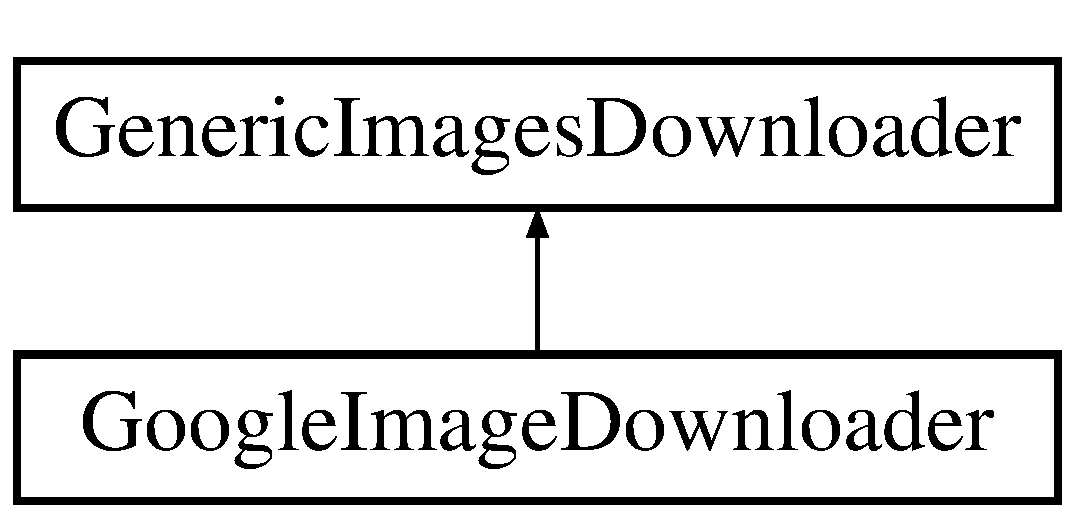
\includegraphics[height=2.000000cm]{class_google_image_downloader}
\end{center}
\end{figure}
\subsection*{Public Member Functions}
\begin{DoxyCompactItemize}
\item 
\hyperlink{class_google_image_downloader_af7a671cb2bc664328fb5224f0da6ef60}{\-\_\-\-\_\-construct} (\$keywords=null)
\begin{DoxyCompactList}\small\item\em Le constructeur. \end{DoxyCompactList}\item 
\hyperlink{class_google_image_downloader_aeaf78020730e78dd35d16d14b527b44c}{search} (array \&\$errors=array())
\begin{DoxyCompactList}\small\item\em Débute une recherche sur google image. \end{DoxyCompactList}\end{DoxyCompactItemize}
\subsection*{Protected Attributes}
\begin{DoxyCompactItemize}
\item 
\hypertarget{class_google_image_downloader_ad9721caaec06f589accb445e1679fb2b}{\hyperlink{class_google_image_downloader_ad9721caaec06f589accb445e1679fb2b}{\$num\-Page} = 0}\label{class_google_image_downloader_ad9721caaec06f589accb445e1679fb2b}

\begin{DoxyCompactList}\small\item\em \$num\-Page Numéro de la page a recherché \end{DoxyCompactList}\item 
\hypertarget{class_google_image_downloader_a8af857b050cdfa3d831eb246f8983cb5}{\hyperlink{class_google_image_downloader_a8af857b050cdfa3d831eb246f8983cb5}{\$img\-Per\-Page} = 20}\label{class_google_image_downloader_a8af857b050cdfa3d831eb246f8983cb5}

\begin{DoxyCompactList}\small\item\em \$img\-Per\-Page Nombre d'image par page de recherche sur le site imagebase.\-net, sert a la création de la pagination \end{DoxyCompactList}\end{DoxyCompactItemize}
\subsection*{Additional Inherited Members}


\subsection{Detailed Description}
Cette classe permet de télécharger les images des résultats de \char`\"{}\-Google Image\char`\"{}. 

\begin{DoxyAuthor}{Author}
M. D. (\href{mailto:mikanono01@hotmail.com}{\tt mikanono01@hotmail.\-com}) 
\end{DoxyAuthor}
\begin{DoxyVersion}{Version}
1 (27/02/2013) 
\end{DoxyVersion}


\subsection{Constructor \& Destructor Documentation}
\hypertarget{class_google_image_downloader_af7a671cb2bc664328fb5224f0da6ef60}{\index{Google\-Image\-Downloader@{Google\-Image\-Downloader}!\-\_\-\-\_\-construct@{\-\_\-\-\_\-construct}}
\index{\-\_\-\-\_\-construct@{\-\_\-\-\_\-construct}!GoogleImageDownloader@{Google\-Image\-Downloader}}
\subsubsection[{\-\_\-\-\_\-construct}]{\setlength{\rightskip}{0pt plus 5cm}\-\_\-\-\_\-construct (
\begin{DoxyParamCaption}
\item[{}]{\$keywords = {\ttfamily null}}
\end{DoxyParamCaption}
)}}\label{class_google_image_downloader_af7a671cb2bc664328fb5224f0da6ef60}


Le constructeur. 


\begin{DoxyParams}{Parameters}
{\em \$keywords} & Chaine de caractères comportant les mots clés.\\
\hline
\end{DoxyParams}
Appel de la fonction setkeywords s'il y a des mots clés. 

\subsection{Member Function Documentation}
\hypertarget{class_google_image_downloader_aeaf78020730e78dd35d16d14b527b44c}{\index{Google\-Image\-Downloader@{Google\-Image\-Downloader}!search@{search}}
\index{search@{search}!GoogleImageDownloader@{Google\-Image\-Downloader}}
\subsubsection[{search}]{\setlength{\rightskip}{0pt plus 5cm}search (
\begin{DoxyParamCaption}
\item[{array \&}]{\$errors = {\ttfamily array()}}
\end{DoxyParamCaption}
)}}\label{class_google_image_downloader_aeaf78020730e78dd35d16d14b527b44c}


Débute une recherche sur google image. 


\begin{DoxyParams}{Parameters}
{\em \$errors} & Un tableau servant a affiché les possibles erreurs. \\
\hline
\end{DoxyParams}
\begin{DoxyReturn}{Returns}
Un nombre entier pour le nombre d'image trouvée ou false en cas de problème. 
\end{DoxyReturn}


The documentation for this class was generated from the following file\-:\begin{DoxyCompactItemize}
\item 
\hyperlink{_google_image_downloader_8class_8php}{Google\-Image\-Downloader.\-class.\-php}\end{DoxyCompactItemize}

\hypertarget{class_imagebase_downloader}{\section{Imagebase\-Downloader Class Reference}
\label{class_imagebase_downloader}\index{Imagebase\-Downloader@{Imagebase\-Downloader}}
}


Cette classe permet de télécharger les images des résultats de \char`\"{}imagebase.\-net\char`\"{}.  


Inheritance diagram for Imagebase\-Downloader\-:\begin{figure}[H]
\begin{center}
\leavevmode
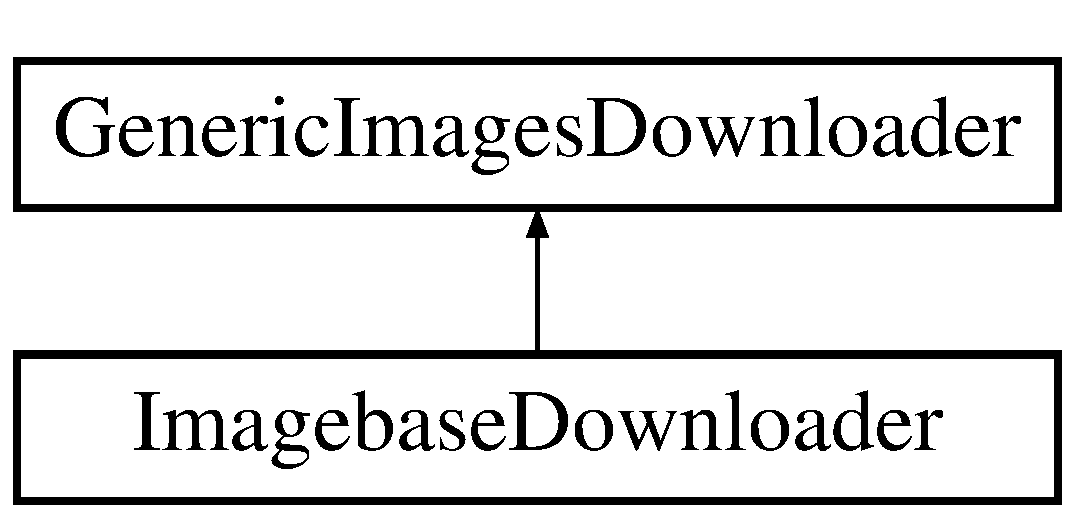
\includegraphics[height=2.000000cm]{class_imagebase_downloader}
\end{center}
\end{figure}
\subsection*{Public Member Functions}
\begin{DoxyCompactItemize}
\item 
\hyperlink{class_imagebase_downloader_af7a671cb2bc664328fb5224f0da6ef60}{\-\_\-\-\_\-construct} (\$keywords=null)
\begin{DoxyCompactList}\small\item\em Le constructeur. \end{DoxyCompactList}\item 
\hyperlink{class_imagebase_downloader_aeaf78020730e78dd35d16d14b527b44c}{search} (array \&\$errors=array())
\begin{DoxyCompactList}\small\item\em Débute une recherche sur photo\-Bucket. \end{DoxyCompactList}\end{DoxyCompactItemize}
\subsection*{Protected Attributes}
\begin{DoxyCompactItemize}
\item 
\hypertarget{class_imagebase_downloader_a8af857b050cdfa3d831eb246f8983cb5}{\hyperlink{class_imagebase_downloader_a8af857b050cdfa3d831eb246f8983cb5}{\$img\-Per\-Page} = 18}\label{class_imagebase_downloader_a8af857b050cdfa3d831eb246f8983cb5}

\begin{DoxyCompactList}\small\item\em \$img\-Per\-Page Nombre d'image par page de recherche sur le site imagebase.\-net, sert a la création de la pagination \end{DoxyCompactList}\end{DoxyCompactItemize}
\subsection*{Additional Inherited Members}


\subsection{Detailed Description}
Cette classe permet de télécharger les images des résultats de \char`\"{}imagebase.\-net\char`\"{}. 

\begin{DoxyAuthor}{Author}
M. D. (\href{mailto:mikanono01@hotmail.com}{\tt mikanono01@hotmail.\-com}) 
\end{DoxyAuthor}
\begin{DoxyVersion}{Version}
1 (27/02/2013) 
\end{DoxyVersion}


\subsection{Constructor \& Destructor Documentation}
\hypertarget{class_imagebase_downloader_af7a671cb2bc664328fb5224f0da6ef60}{\index{Imagebase\-Downloader@{Imagebase\-Downloader}!\-\_\-\-\_\-construct@{\-\_\-\-\_\-construct}}
\index{\-\_\-\-\_\-construct@{\-\_\-\-\_\-construct}!ImagebaseDownloader@{Imagebase\-Downloader}}
\subsubsection[{\-\_\-\-\_\-construct}]{\setlength{\rightskip}{0pt plus 5cm}\-\_\-\-\_\-construct (
\begin{DoxyParamCaption}
\item[{}]{\$keywords = {\ttfamily null}}
\end{DoxyParamCaption}
)}}\label{class_imagebase_downloader_af7a671cb2bc664328fb5224f0da6ef60}


Le constructeur. 


\begin{DoxyParams}{Parameters}
{\em \$keywords} & Chaine de caractères comportant les mots clés.\\
\hline
\end{DoxyParams}
Appel de la fonction setkeywords s'il y a des mots clés. 

\subsection{Member Function Documentation}
\hypertarget{class_imagebase_downloader_aeaf78020730e78dd35d16d14b527b44c}{\index{Imagebase\-Downloader@{Imagebase\-Downloader}!search@{search}}
\index{search@{search}!ImagebaseDownloader@{Imagebase\-Downloader}}
\subsubsection[{search}]{\setlength{\rightskip}{0pt plus 5cm}search (
\begin{DoxyParamCaption}
\item[{array \&}]{\$errors = {\ttfamily array()}}
\end{DoxyParamCaption}
)}}\label{class_imagebase_downloader_aeaf78020730e78dd35d16d14b527b44c}


Débute une recherche sur photo\-Bucket. 


\begin{DoxyParams}{Parameters}
{\em \$errors} & Un tableau servant a affiché les possibles erreurs. \\
\hline
\end{DoxyParams}
\begin{DoxyReturn}{Returns}
Un nombre entier pour le nombre d'image trouvée ou false en cas de problème. 
\end{DoxyReturn}


The documentation for this class was generated from the following file\-:\begin{DoxyCompactItemize}
\item 
\hyperlink{_image_base_downloader_8class_8php}{Image\-Base\-Downloader.\-class.\-php}\end{DoxyCompactItemize}

\hypertarget{class_office_image_downloader}{\section{Office\-Image\-Downloader Class Reference}
\label{class_office_image_downloader}\index{Office\-Image\-Downloader@{Office\-Image\-Downloader}}
}


Cette classe permet de télécharger les images des résultats de \char`\"{}\-Office.\-microsoft.\-com\char`\"{}.  


Inheritance diagram for Office\-Image\-Downloader\-:\begin{figure}[H]
\begin{center}
\leavevmode
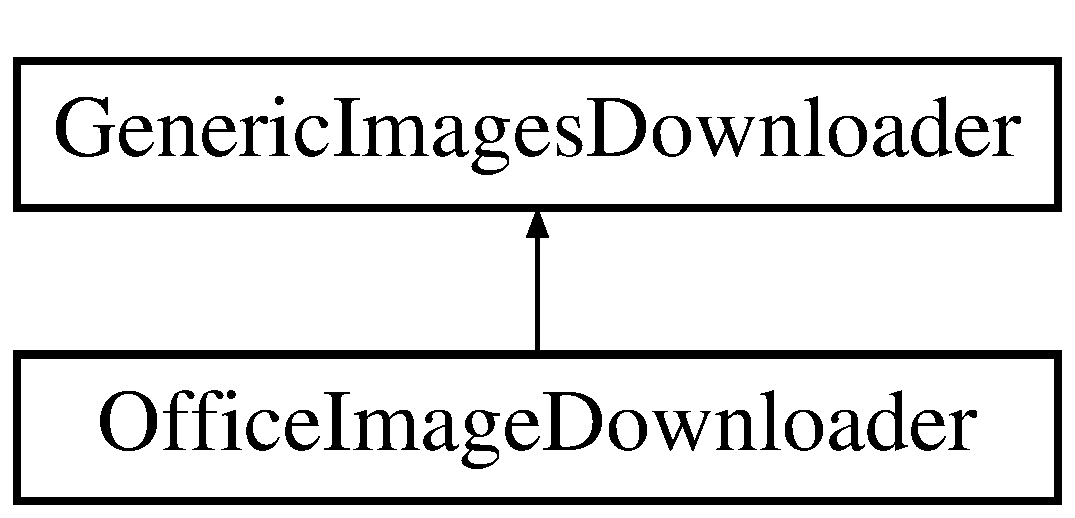
\includegraphics[height=2.000000cm]{class_office_image_downloader}
\end{center}
\end{figure}
\subsection*{Public Member Functions}
\begin{DoxyCompactItemize}
\item 
\hyperlink{class_office_image_downloader_af7a671cb2bc664328fb5224f0da6ef60}{\-\_\-\-\_\-construct} (\$keywords=null)
\begin{DoxyCompactList}\small\item\em Le constructeur. \end{DoxyCompactList}\item 
\hyperlink{class_office_image_downloader_aeaf78020730e78dd35d16d14b527b44c}{search} (array \&\$errors=array())
\begin{DoxyCompactList}\small\item\em Débute une recherche sur Microsoft office. \end{DoxyCompactList}\end{DoxyCompactItemize}
\subsection*{Protected Member Functions}
\begin{DoxyCompactItemize}
\item 
\hypertarget{class_office_image_downloader_a3a3e8ed69a7a72d69950426ec9424a64}{\hyperlink{class_office_image_downloader_a3a3e8ed69a7a72d69950426ec9424a64}{build\-U\-R\-L} ()}\label{class_office_image_downloader_a3a3e8ed69a7a72d69950426ec9424a64}

\begin{DoxyCompactList}\small\item\em Fonction permettant la création de l'U\-R\-L. \end{DoxyCompactList}\end{DoxyCompactItemize}
\subsection*{Additional Inherited Members}


\subsection{Detailed Description}
Cette classe permet de télécharger les images des résultats de \char`\"{}\-Office.\-microsoft.\-com\char`\"{}. 

\begin{DoxyAuthor}{Author}
M. D. (\href{mailto:mikanono01@hotmail.com}{\tt mikanono01@hotmail.\-com}) 
\end{DoxyAuthor}
\begin{DoxyVersion}{Version}
1 (27/02/2013) 
\end{DoxyVersion}


\subsection{Constructor \& Destructor Documentation}
\hypertarget{class_office_image_downloader_af7a671cb2bc664328fb5224f0da6ef60}{\index{Office\-Image\-Downloader@{Office\-Image\-Downloader}!\-\_\-\-\_\-construct@{\-\_\-\-\_\-construct}}
\index{\-\_\-\-\_\-construct@{\-\_\-\-\_\-construct}!OfficeImageDownloader@{Office\-Image\-Downloader}}
\subsubsection[{\-\_\-\-\_\-construct}]{\setlength{\rightskip}{0pt plus 5cm}\-\_\-\-\_\-construct (
\begin{DoxyParamCaption}
\item[{}]{\$keywords = {\ttfamily null}}
\end{DoxyParamCaption}
)}}\label{class_office_image_downloader_af7a671cb2bc664328fb5224f0da6ef60}


Le constructeur. 


\begin{DoxyParams}{Parameters}
{\em \$keywords} & Chaine de caractères comportant les mots clés.\\
\hline
\end{DoxyParams}
Appel de la fonction setkeywords s'il y a des mots clés. 

\subsection{Member Function Documentation}
\hypertarget{class_office_image_downloader_aeaf78020730e78dd35d16d14b527b44c}{\index{Office\-Image\-Downloader@{Office\-Image\-Downloader}!search@{search}}
\index{search@{search}!OfficeImageDownloader@{Office\-Image\-Downloader}}
\subsubsection[{search}]{\setlength{\rightskip}{0pt plus 5cm}search (
\begin{DoxyParamCaption}
\item[{array \&}]{\$errors = {\ttfamily array()}}
\end{DoxyParamCaption}
)}}\label{class_office_image_downloader_aeaf78020730e78dd35d16d14b527b44c}


Débute une recherche sur Microsoft office. 


\begin{DoxyParams}{Parameters}
{\em \$errors} & Un tableau servant a affiché les possibles erreurs. \\
\hline
\end{DoxyParams}
\begin{DoxyReturn}{Returns}
Un nombre entier pour le nombre d'image trouvée ou false en cas de problème. 
\end{DoxyReturn}


The documentation for this class was generated from the following file\-:\begin{DoxyCompactItemize}
\item 
\hyperlink{_office_image_downloader_8class_8php}{Office\-Image\-Downloader.\-class.\-php}\end{DoxyCompactItemize}

\hypertarget{class_photo_bucket_downloader}{\section{Photo\-Bucket\-Downloader Class Reference}
\label{class_photo_bucket_downloader}\index{Photo\-Bucket\-Downloader@{Photo\-Bucket\-Downloader}}
}


Cette classe permet de télécharger les images des résultats de \char`\"{}photobucket.\-com\char`\"{}.  


Inheritance diagram for Photo\-Bucket\-Downloader\-:\begin{figure}[H]
\begin{center}
\leavevmode
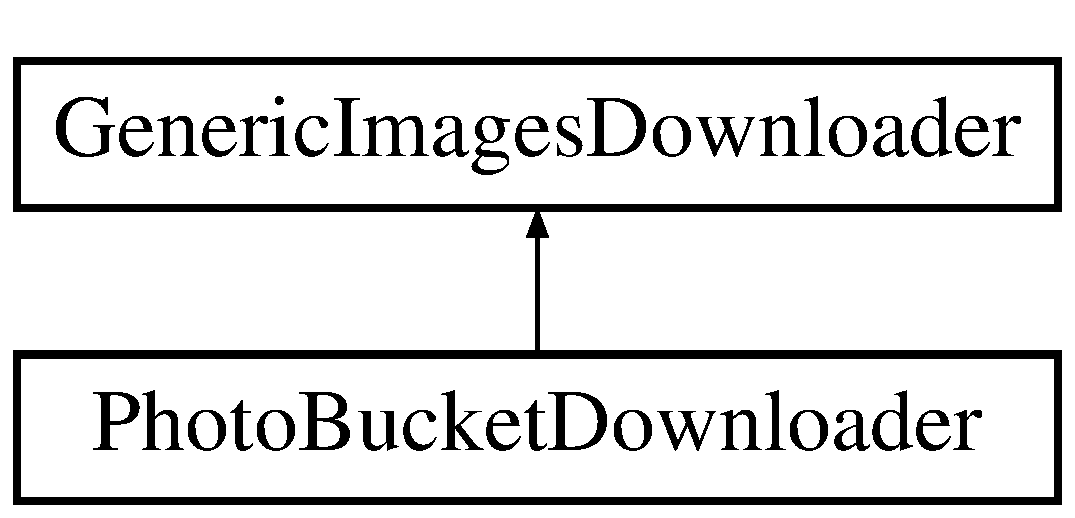
\includegraphics[height=2.000000cm]{class_photo_bucket_downloader}
\end{center}
\end{figure}
\subsection*{Public Member Functions}
\begin{DoxyCompactItemize}
\item 
\hyperlink{class_photo_bucket_downloader_af7a671cb2bc664328fb5224f0da6ef60}{\-\_\-\-\_\-construct} (\$keywords=null)
\begin{DoxyCompactList}\small\item\em Le constructeur. \end{DoxyCompactList}\item 
\hyperlink{class_photo_bucket_downloader_aeaf78020730e78dd35d16d14b527b44c}{search} (array \&\$errors=array())
\begin{DoxyCompactList}\small\item\em Débute une recherche sur photo\-Bucket. \end{DoxyCompactList}\end{DoxyCompactItemize}
\subsection*{Additional Inherited Members}


\subsection{Detailed Description}
Cette classe permet de télécharger les images des résultats de \char`\"{}photobucket.\-com\char`\"{}. 

\begin{DoxyAuthor}{Author}
M. D. (\href{mailto:mikanono01@hotmail.com}{\tt mikanono01@hotmail.\-com}) 
\end{DoxyAuthor}
\begin{DoxyVersion}{Version}
1 (27/02/2013) 
\end{DoxyVersion}


\subsection{Constructor \& Destructor Documentation}
\hypertarget{class_photo_bucket_downloader_af7a671cb2bc664328fb5224f0da6ef60}{\index{Photo\-Bucket\-Downloader@{Photo\-Bucket\-Downloader}!\-\_\-\-\_\-construct@{\-\_\-\-\_\-construct}}
\index{\-\_\-\-\_\-construct@{\-\_\-\-\_\-construct}!PhotoBucketDownloader@{Photo\-Bucket\-Downloader}}
\subsubsection[{\-\_\-\-\_\-construct}]{\setlength{\rightskip}{0pt plus 5cm}\-\_\-\-\_\-construct (
\begin{DoxyParamCaption}
\item[{}]{\$keywords = {\ttfamily null}}
\end{DoxyParamCaption}
)}}\label{class_photo_bucket_downloader_af7a671cb2bc664328fb5224f0da6ef60}


Le constructeur. 


\begin{DoxyParams}{Parameters}
{\em \$keywords} & Chaine de caractères comportant les mots clés.\\
\hline
\end{DoxyParams}
Appel de la fonction setkeywords s'il y a des mots clés. 

\subsection{Member Function Documentation}
\hypertarget{class_photo_bucket_downloader_aeaf78020730e78dd35d16d14b527b44c}{\index{Photo\-Bucket\-Downloader@{Photo\-Bucket\-Downloader}!search@{search}}
\index{search@{search}!PhotoBucketDownloader@{Photo\-Bucket\-Downloader}}
\subsubsection[{search}]{\setlength{\rightskip}{0pt plus 5cm}search (
\begin{DoxyParamCaption}
\item[{array \&}]{\$errors = {\ttfamily array()}}
\end{DoxyParamCaption}
)}}\label{class_photo_bucket_downloader_aeaf78020730e78dd35d16d14b527b44c}


Débute une recherche sur photo\-Bucket. 


\begin{DoxyParams}{Parameters}
{\em \$errors} & Un tableau servant a affiché les possibles erreurs. \\
\hline
\end{DoxyParams}
\begin{DoxyReturn}{Returns}
Un nombre entier pour le nombre d'image trouvée ou false en cas de problème. 
\end{DoxyReturn}


The documentation for this class was generated from the following file\-:\begin{DoxyCompactItemize}
\item 
\hyperlink{_photo_bucket_downloader_8class_8php}{Photo\-Bucket\-Downloader.\-class.\-php}\end{DoxyCompactItemize}

\hypertarget{class_rgb_stock_image_downloader}{\section{Rgb\-Stock\-Image\-Downloader Class Reference}
\label{class_rgb_stock_image_downloader}\index{Rgb\-Stock\-Image\-Downloader@{Rgb\-Stock\-Image\-Downloader}}
}


Cette classe permet de télécharger les images des résultats de \char`\"{}rgbstock.\-com\char`\"{}.  


Inheritance diagram for Rgb\-Stock\-Image\-Downloader\-:\begin{figure}[H]
\begin{center}
\leavevmode
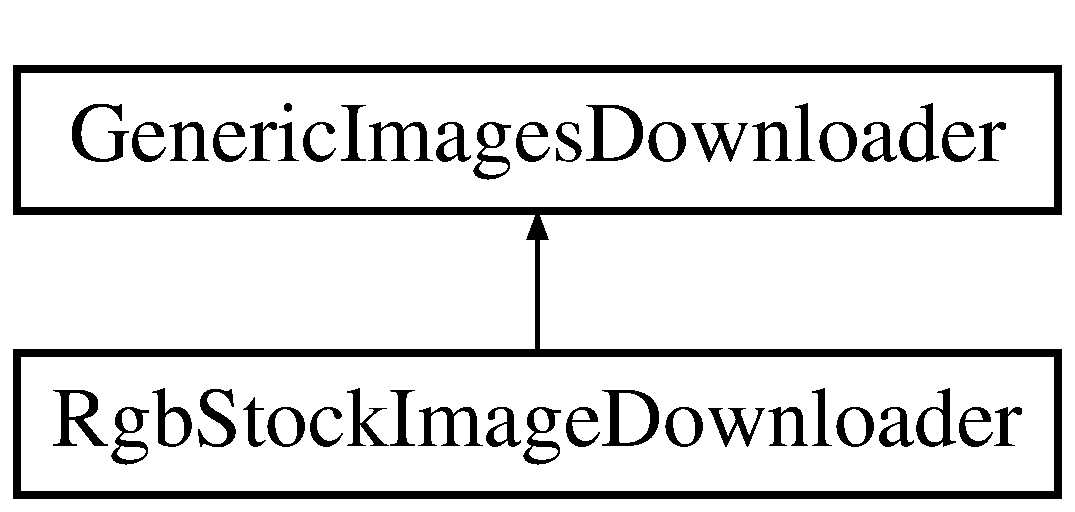
\includegraphics[height=2.000000cm]{class_rgb_stock_image_downloader}
\end{center}
\end{figure}
\subsection*{Public Member Functions}
\begin{DoxyCompactItemize}
\item 
\hyperlink{class_rgb_stock_image_downloader_af7a671cb2bc664328fb5224f0da6ef60}{\-\_\-\-\_\-construct} (\$keywords=null)
\begin{DoxyCompactList}\small\item\em Le constructeur. \end{DoxyCompactList}\item 
\hyperlink{class_rgb_stock_image_downloader_aeaf78020730e78dd35d16d14b527b44c}{search} (array \&\$errors=array())
\begin{DoxyCompactList}\small\item\em Débute une recherche sur photo\-Bucket. \end{DoxyCompactList}\end{DoxyCompactItemize}
\subsection*{Additional Inherited Members}


\subsection{Detailed Description}
Cette classe permet de télécharger les images des résultats de \char`\"{}rgbstock.\-com\char`\"{}. 

\begin{DoxyAuthor}{Author}
M. D. (\href{mailto:mikanono01@hotmail.com}{\tt mikanono01@hotmail.\-com}) 
\end{DoxyAuthor}
\begin{DoxyVersion}{Version}
1 (27/02/2013) 
\end{DoxyVersion}


\subsection{Constructor \& Destructor Documentation}
\hypertarget{class_rgb_stock_image_downloader_af7a671cb2bc664328fb5224f0da6ef60}{\index{Rgb\-Stock\-Image\-Downloader@{Rgb\-Stock\-Image\-Downloader}!\-\_\-\-\_\-construct@{\-\_\-\-\_\-construct}}
\index{\-\_\-\-\_\-construct@{\-\_\-\-\_\-construct}!RgbStockImageDownloader@{Rgb\-Stock\-Image\-Downloader}}
\subsubsection[{\-\_\-\-\_\-construct}]{\setlength{\rightskip}{0pt plus 5cm}\-\_\-\-\_\-construct (
\begin{DoxyParamCaption}
\item[{}]{\$keywords = {\ttfamily null}}
\end{DoxyParamCaption}
)}}\label{class_rgb_stock_image_downloader_af7a671cb2bc664328fb5224f0da6ef60}


Le constructeur. 


\begin{DoxyParams}{Parameters}
{\em \$keywords} & Chaine de caractères comportant les mots clés.\\
\hline
\end{DoxyParams}
Appel de la fonction setkeywords s'il y a des mots clés. 

\subsection{Member Function Documentation}
\hypertarget{class_rgb_stock_image_downloader_aeaf78020730e78dd35d16d14b527b44c}{\index{Rgb\-Stock\-Image\-Downloader@{Rgb\-Stock\-Image\-Downloader}!search@{search}}
\index{search@{search}!RgbStockImageDownloader@{Rgb\-Stock\-Image\-Downloader}}
\subsubsection[{search}]{\setlength{\rightskip}{0pt plus 5cm}search (
\begin{DoxyParamCaption}
\item[{array \&}]{\$errors = {\ttfamily array()}}
\end{DoxyParamCaption}
)}}\label{class_rgb_stock_image_downloader_aeaf78020730e78dd35d16d14b527b44c}


Débute une recherche sur photo\-Bucket. 


\begin{DoxyParams}{Parameters}
{\em \$errors} & Un tableau servant a affiché les possibles erreurs. \\
\hline
\end{DoxyParams}
\begin{DoxyReturn}{Returns}
Un nombre entier pour le nombre d'image trouvée ou false en cas de problème. 
\end{DoxyReturn}


The documentation for this class was generated from the following file\-:\begin{DoxyCompactItemize}
\item 
\hyperlink{_rgb_stock_image_downloader_8class_8php}{Rgb\-Stock\-Image\-Downloader.\-class.\-php}\end{DoxyCompactItemize}

\chapter{File Documentation}
\hypertarget{_generic_images_downloader_8class_8php}{\section{Generic\-Images\-Downloader.\-class.\-php File Reference}
\label{_generic_images_downloader_8class_8php}\index{Generic\-Images\-Downloader.\-class.\-php@{Generic\-Images\-Downloader.\-class.\-php}}
}


\hyperlink{class_generic_images_downloader}{Generic\-Images\-Downloader} class file.  


\subsection*{Data Structures}
\begin{DoxyCompactItemize}
\item 
class \hyperlink{class_generic_images_downloader}{Generic\-Images\-Downloader}
\begin{DoxyCompactList}\small\item\em Cette classe est la classe générique à toutes les auutres. \end{DoxyCompactList}\end{DoxyCompactItemize}


\subsection{Detailed Description}
\hyperlink{class_generic_images_downloader}{Generic\-Images\-Downloader} class file. \begin{DoxyAuthor}{Author}
M. D. (\href{mailto:mikanono01@hotmail.com}{\tt mikanono01@hotmail.\-com}) 
\end{DoxyAuthor}
\begin{DoxyVersion}{Version}
1 (27/02/2013) Classe générique à toute les autres classes 
\end{DoxyVersion}

\hypertarget{googleimage_8class_8php}{\section{googleimage.\-class.\-php File Reference}
\label{googleimage_8class_8php}\index{googleimage.\-class.\-php@{googleimage.\-class.\-php}}
}


\hyperlink{class_google_image}{Google\-Image} class file.  


\subsection*{Data Structures}
\begin{DoxyCompactItemize}
\item 
class \hyperlink{class_google_image}{Google\-Image}
\begin{DoxyCompactList}\small\item\em Cette classe permet de télécharger les images des résultats de \char`\"{}\-Google Image\char`\"{}. \end{DoxyCompactList}\end{DoxyCompactItemize}


\subsection{Detailed Description}
\hyperlink{class_google_image}{Google\-Image} class file. \begin{DoxyAuthor}{Author}
Lond\-Noir (\href{mailto:londnoir@sdmedia.be}{\tt londnoir@sdmedia.\-be}) 
\end{DoxyAuthor}
\begin{DoxyVersion}{Version}
1.\-2 (24/04/2012) 
\end{DoxyVersion}

\hypertarget{_google_image_downloader_8class_8php}{\section{Google\-Image\-Downloader.\-class.\-php File Reference}
\label{_google_image_downloader_8class_8php}\index{Google\-Image\-Downloader.\-class.\-php@{Google\-Image\-Downloader.\-class.\-php}}
}


\hyperlink{class_google_image_downloader}{Google\-Image\-Downloader} class file.  


\subsection*{Data Structures}
\begin{DoxyCompactItemize}
\item 
class \hyperlink{class_google_image_downloader}{Google\-Image\-Downloader}
\begin{DoxyCompactList}\small\item\em Cette classe permet de télécharger les images des résultats de \char`\"{}\-Google Image\char`\"{}. \end{DoxyCompactList}\end{DoxyCompactItemize}


\subsection{Detailed Description}
\hyperlink{class_google_image_downloader}{Google\-Image\-Downloader} class file. \begin{DoxyAuthor}{Author}
M. D. (\href{mailto:mikanono01@hotmail.com}{\tt mikanono01@hotmail.\-com}) 
\end{DoxyAuthor}
\begin{DoxyVersion}{Version}
1 (27/02/2013) 
\end{DoxyVersion}

\hypertarget{_image_base_downloader_8class_8php}{\section{Image\-Base\-Downloader.\-class.\-php File Reference}
\label{_image_base_downloader_8class_8php}\index{Image\-Base\-Downloader.\-class.\-php@{Image\-Base\-Downloader.\-class.\-php}}
}


\hyperlink{class_imagebase_downloader}{Imagebase\-Downloader} class file.  


\subsection*{Data Structures}
\begin{DoxyCompactItemize}
\item 
class \hyperlink{class_imagebase_downloader}{Imagebase\-Downloader}
\begin{DoxyCompactList}\small\item\em Cette classe permet de télécharger les images des résultats de \char`\"{}imagebase.\-net\char`\"{}. \end{DoxyCompactList}\end{DoxyCompactItemize}


\subsection{Detailed Description}
\hyperlink{class_imagebase_downloader}{Imagebase\-Downloader} class file. \begin{DoxyAuthor}{Author}
M. D. (\href{mailto:mikanono01@hotmail.com}{\tt mikanono01@hotmail.\-com}) 
\end{DoxyAuthor}
\begin{DoxyVersion}{Version}
1 (27/02/2013) 
\end{DoxyVersion}

\hypertarget{_office_image_downloader_8class_8php}{\section{Office\-Image\-Downloader.\-class.\-php File Reference}
\label{_office_image_downloader_8class_8php}\index{Office\-Image\-Downloader.\-class.\-php@{Office\-Image\-Downloader.\-class.\-php}}
}


\hyperlink{class_office_image_downloader}{Office\-Image\-Downloader} class file.  


\subsection*{Data Structures}
\begin{DoxyCompactItemize}
\item 
class \hyperlink{class_office_image_downloader}{Office\-Image\-Downloader}
\begin{DoxyCompactList}\small\item\em Cette classe permet de télécharger les images des résultats de \char`\"{}\-Office.\-microsoft.\-com\char`\"{}. \end{DoxyCompactList}\end{DoxyCompactItemize}


\subsection{Detailed Description}
\hyperlink{class_office_image_downloader}{Office\-Image\-Downloader} class file. \begin{DoxyAuthor}{Author}
M. D. (\href{mailto:mikanono01@hotmail.com}{\tt mikanono01@hotmail.\-com}) 
\end{DoxyAuthor}
\begin{DoxyVersion}{Version}
1 (27/02/2013) 
\end{DoxyVersion}

\hypertarget{_photo_bucket_downloader_8class_8php}{\section{Photo\-Bucket\-Downloader.\-class.\-php File Reference}
\label{_photo_bucket_downloader_8class_8php}\index{Photo\-Bucket\-Downloader.\-class.\-php@{Photo\-Bucket\-Downloader.\-class.\-php}}
}


\hyperlink{class_photo_bucket_downloader}{Photo\-Bucket\-Downloader} class file.  


\subsection*{Data Structures}
\begin{DoxyCompactItemize}
\item 
class \hyperlink{class_photo_bucket_downloader}{Photo\-Bucket\-Downloader}
\begin{DoxyCompactList}\small\item\em Cette classe permet de télécharger les images des résultats de \char`\"{}photobucket.\-com\char`\"{}. \end{DoxyCompactList}\end{DoxyCompactItemize}


\subsection{Detailed Description}
\hyperlink{class_photo_bucket_downloader}{Photo\-Bucket\-Downloader} class file. \begin{DoxyAuthor}{Author}
M. D. (\href{mailto:mikanono01@hotmail.com}{\tt mikanono01@hotmail.\-com}) 
\end{DoxyAuthor}
\begin{DoxyVersion}{Version}
1 (27/02/2013) 
\end{DoxyVersion}

\hypertarget{_rgb_stock_image_downloader_8class_8php}{\section{Rgb\-Stock\-Image\-Downloader.\-class.\-php File Reference}
\label{_rgb_stock_image_downloader_8class_8php}\index{Rgb\-Stock\-Image\-Downloader.\-class.\-php@{Rgb\-Stock\-Image\-Downloader.\-class.\-php}}
}


\hyperlink{class_rgb_stock_image_downloader}{Rgb\-Stock\-Image\-Downloader} class file.  


\subsection*{Data Structures}
\begin{DoxyCompactItemize}
\item 
class \hyperlink{class_rgb_stock_image_downloader}{Rgb\-Stock\-Image\-Downloader}
\begin{DoxyCompactList}\small\item\em Cette classe permet de télécharger les images des résultats de \char`\"{}rgbstock.\-com\char`\"{}. \end{DoxyCompactList}\end{DoxyCompactItemize}


\subsection{Detailed Description}
\hyperlink{class_rgb_stock_image_downloader}{Rgb\-Stock\-Image\-Downloader} class file. \begin{DoxyAuthor}{Author}
M. D. (\href{mailto:mikanono01@hotmail.com}{\tt mikanono01@hotmail.\-com}) 
\end{DoxyAuthor}
\begin{DoxyVersion}{Version}
1 (27/02/2013) 
\end{DoxyVersion}

\addcontentsline{toc}{part}{Index}
\printindex
\end{document}
